\chapter{Depletion Capacitance and Doping Profiling}
\label{ch:depletion-capacitance}

A reverse-biased junction stores equal and opposite fixed charge on its two
sides.  Changing voltage moves the depletion edges and changes that charge.
The incremental charge response is the depletion capacitance.  Because the
moving edge samples the local dopant density, capacitance--voltage measurement
also becomes a spatial profiling method \cite[Chap.~3, Sec.~3.3]{szeLee2012}.

\section{Definitions and units}

\begin{definition}{Junction depletion capacitance}{junction-capacitance}
Let $Q$ be the magnitude of depletion charge per unit area in
$\mathrm{C\,m^{-2}}$.  The depletion capacitance per unit area is
\begin{equation}
  C_j\equiv\left|\frac{\dd Q}{\dd V}\right|,
  \label{eq:depletion-capacitance-definition}
\end{equation}
measured in $\mathrm{F\,m^{-2}}$.  Device capacitance is $A_jC_j$, where $A_j$
is junction area in square meters.
\end{definition}

The derivative is a small-signal quantity about a specified DC bias.  It is not
the ratio $Q/V$.  Reverse-bias magnitude is denoted $V_R=-V\ge0$.

\section{Abrupt-junction capacitance}

For a differential change, the incremental field occupies approximately the
entire depletion width.  Gauss's law then gives
\begin{equation}
  \boxed{C_j=\frac{\varepsilon_s}{W}.}
  \label{eq:depletion-capacitance-width}
\end{equation}
Combining this result with \cref{eq:pn-abrupt-width} yields
\begin{equation}
 C_j=
 \left[
 \frac{q\varepsilon_sN_AN_D}
 {2(N_A+N_D)(V_{\mathrm{bi}}+V_R)}
 \right]^{1/2}.
 \label{eq:abrupt-capacitance}
\end{equation}
Thus reverse bias widens the layer and lowers capacitance.  For a one-sided
$p^+$--n junction,
\begin{equation}
 \frac{1}{C_j^2}
 =\frac{2(V_{\mathrm{bi}}+V_R)}{q\varepsilon_sN_D}.
 \label{eq:one-sided-cv-linear}
\end{equation}
A plot of $1/C_j^2$ against $V_R$ is linear.  Its slope determines $N_D$ and
its voltage-axis intercept determines $-V_{\mathrm{bi}}$.

For the linearly graded profile of \cref{eq:pn-graded-width},
\begin{equation}
 C_j=\frac{\varepsilon_s}{W}
 =\left[
 \frac{q a\varepsilon_s^2}{12(V_{\mathrm{bi}}+V_R)}
 \right]^{1/3}.
 \label{eq:graded-capacitance}
\end{equation}
Consequently $1/C_j^3$, rather than $1/C_j^2$, is linear in voltage.

\section{Doping extraction}

For an arbitrary one-sided profile, a small increase $\dd W$ uncovers charge
$\dd Q=qN(W)\dd W$.  The incremental voltage associated with the field change
leads to
\begin{equation}
 \boxed{
 N(W)=\frac{2}{q\varepsilon_s}
 \left[\frac{\dd(1/C_j^2)}{\dd V_R}\right]^{-1},
 \qquad
 W=\frac{\varepsilon_s}{C_j}.
 }
 \label{eq:cv-doping-profile}
\end{equation}
Here $N(W)$ is the dopant density at the moving depletion edge in
$\mathrm{m^{-3}}$.  The voltage derivative amplifies experimental noise;
smoothing, uncertainty propagation, and finite probe resolution must accompany
real extraction.

\section{Voltage-variable capacitance}

A reverse-biased diode used as a voltage-controlled capacitor is a varactor.
A useful empirical law is
\begin{equation}
 C_j(V_R)=\frac{C_{j0}}
 {(1+V_R/V_{\mathrm{bi}})^m},
 \label{eq:varactor-law}
\end{equation}
where $m=1/2$ for an abrupt junction and $m=1/3$ for a linearly graded
junction.  A deliberately hyperabrupt profile can produce $m>1/2$ and a wider
capacitance tuning range \cite[Sec.~3.3.3]{szeLee2012}.

\begin{figure}[htbp]
 \centering
 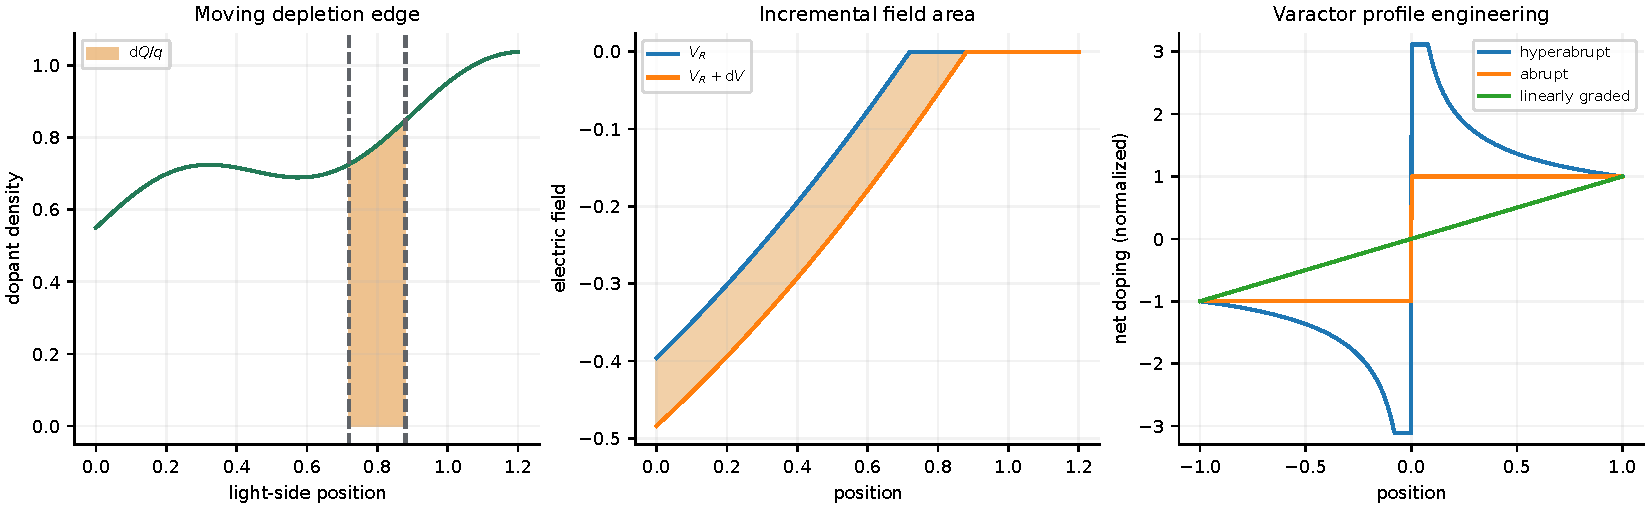
\includegraphics[width=\textwidth]{figures/junction-atlas-capacitance-construction.pdf}
 \caption{Original construction of incremental depletion charge and field,
 together with hyperabrupt, abrupt, and linearly graded varactor profiles.  The
 panels cover the physical content of Figs.~11--13 in Sze--Lee Chapter~3
 \cite[Sec.~3.3]{szeLee2012}.\figurenotebookmark}
 \label{fig:junction-atlas-capacitance-construction}
\end{figure}
\figurenotebooktext{figures/17_depletion-capacitance-profiling/fig_17_01.ipynb}

\section{Numerical differentiation and validation}

The notebook computes $C_j(V_R)$ directly from the analytic depletion width,
forms $1/C_j^2$, and evaluates \cref{eq:cv-doping-profile} with a centered
finite-difference derivative.  For exact abrupt-junction data, the recovered
light-side doping should be independent of voltage.  Grid refinement checks
that derivative error decreases before roundoff or measurement noise dominates.

\begin{figure}[htbp]
 \centering
 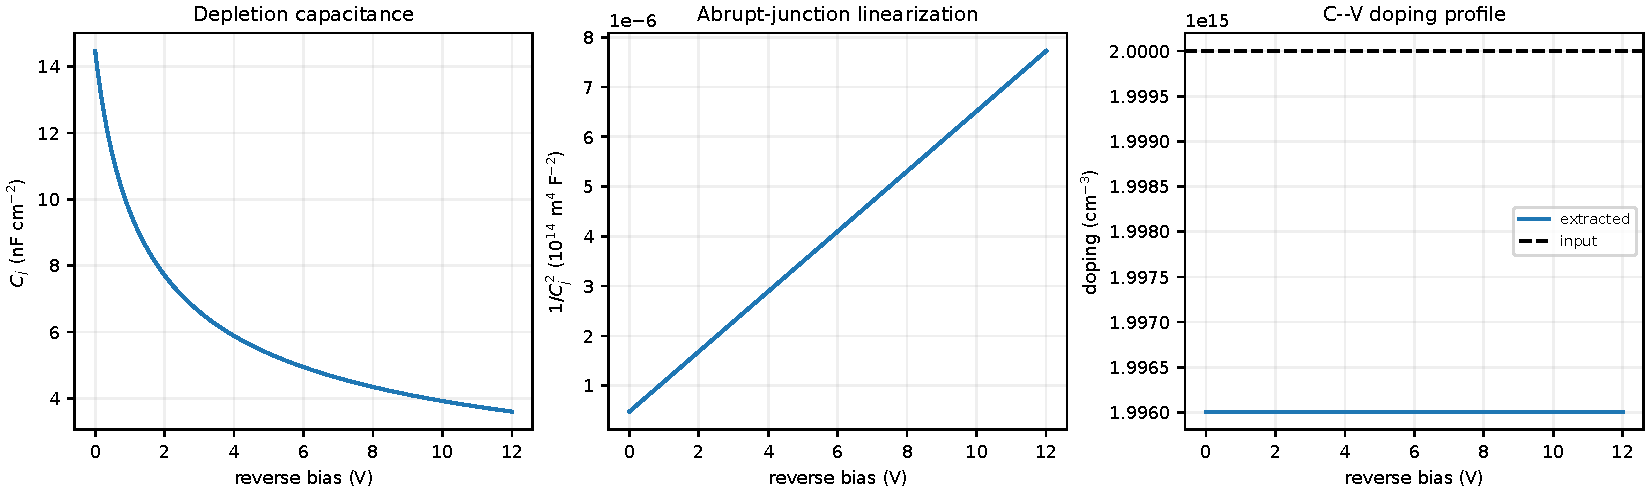
\includegraphics[width=\textwidth]{figures/junction-capacitance-profiling.pdf}
 \caption{Depletion capacitance, abrupt-junction $1/C_j^2$ linearization, and
 numerical recovery of the lightly doped concentration.  The computation uses
 capacitance per unit area throughout.\figurenotebookmark}
 \label{fig:junction-capacitance-profiling}
\end{figure}
\figurenotebooktext{figures/17_depletion-capacitance-profiling/fig_17_01.ipynb}

\begin{modelcheck}
For $N_A\gg N_D$, the finite-difference slope of $1/C_j^2$ recovers $N_D$
within the small correction factor $N_A/(N_A+N_D)$.  The identity
$C_jW=\varepsilon_s$ holds at every bias, and $C_j$ decreases monotonically
with $V_R$.
\end{modelcheck}

\begin{boundarybox}
Series resistance, interface states, deep-level response times, parasitic
capacitance, freeze-out, and mobile-carrier response can distort measured
C--V curves.  The depletion formula assumes the measurement frequency is high
enough to exclude slow minority-carrier redistribution but low enough that the
junction charge follows the excitation quasi-statically.
\end{boundarybox}

\section{Chapter summary}

Depletion capacitance is an incremental charge derivative.  In a planar
junction it equals $\varepsilon_s/W$, so its voltage dependence reveals the
junction profile.  Abrupt junctions linearize as $1/C_j^2$; linearly graded
junctions linearize as $1/C_j^3$.  Numerical differentiation converts C--V data
into a spatial dopant profile but also exposes the method's sensitivity to
noise and nonideal response.
